\documentclass{article}
\usepackage[utf8]{inputenc}
\usepackage{indentfirst}
\usepackage{titling}
\usepackage{geometry}
\usepackage{graphicx}
\graphicspath{ {./Images/} }
\usepackage[shortlabels]{enumitem}
\usepackage{fancyhdr}
\usepackage{ulem}
\usepackage[dvipsnames]{xcolor}
\usepackage{amssymb}

\def\ojoin{\setbox0=\hbox{$\bowtie$}%
  \rule[-.02ex]{.25em}{.4pt}\llap{\rule[\ht0]{.25em}{.4pt}}}
\def\leftouterjoin{\mathbin{\ojoin\mkern-5.8mu\bowtie}}
\def\rightouterjoin{\mathbin{\bowtie\mkern-5.8mu\ojoin}}
\def\fullouterjoin{\mathbin{\ojoin\mkern-5.8mu\bowtie\mkern-5.8mu\ojoin}}

\renewcommand\maketitlehooka{\null\mbox{}\vfill} %para centralizar verticalmente
\renewcommand\maketitlehookd{\vfill\null}
\pagestyle{fancy}
\fancyhf{}
\rfoot{\thepage}
\lfoot{ 
\includegraphics[scale=0.01]{UA.jpg} José Mendes 107188 LEI}
\geometry{
  a4paper,
  headheight=4cm,
  top=5.5cm,
  bottom=4.5cm,
  footskip=4cm
}


\title{Complementos de Bases de Dados}
\author{José Mendes 107188}
\date{2023}

\begin{document}


\begin{titlepage}
    \maketitle
    \begin{center}
        
\includegraphics[scale=0.4]{UA.png}
    \end{center}
    \thispagestyle{empty} %remove o count da pagina
\end{titlepage}

\pagebreak
%depois por um index aqui

\section{Evolução dos Sistemas de Base de Dados}

\begin{flushleft}
    \textbf{Sistemas de Dados -} Cada vez mais as aplicações de hoje em dia
    são Data-Intensive, em vez de Compute-Intensive. 

    Para Data-Intensive, o poder bruto da CPU deixa de ser um fator limitante
    quando comparado com a \textbf{quantidade}, \textbf{complexidade} e \textbf{velocidade de atualização} dos dados.

    \vspace{3mm}

    De forma a otimizar a sua performance, um sistema de dados tipicamente oferece as seguintes
    funcionalidades:
    \begin{enumerate}
      \item \textbf{Bases de Dados -} armazenam os dados para utilização futura;
      \item \textbf{Caches -} guardam os resultados de operações dispendiosas, de forma a tornar a leitura mais rápida;
      \item \textbf{Search Indexes -} permitem aos utilizadores procurarem por palavras-chave ou filtrar os dados;
      \item \textbf{Message Queues -} permitem a comunicação assíncrona entre processos;
      \item \textbf{Stream Processing -} permite o processamento de dados em tempo real;
      \item \textbf{Batch Processing -} permite o processamento de dados acumulados, periodicamente;
    \end{enumerate}

    \textcolor{Blue}{Exemplo:}
    Um exemplo de \textbf{stream processing} ocorre na banca. Sempre que é realizada uma transação, os dados da mesma são
  imediatamente processados de forma a que o saldo esteja sempre atualizado.


  O \textbf{batch processing} é visível na faturação dos serviços pós-pagos pelas operadoras de telecomunicações. No final de
  cada mês, é feita uma consulta às suas bases de dados de forma a identificar todos os consumos do cliente, que são
  somados e depois gerada a fatura.


  No \textbf{stream} os dados são processados antes de armazenados, enquanto que no \textbf{batch} são processados depois de
  armazenados.

  \vspace{3mm}

  Cada vez mais as aplicações requerem um \textbf{maior wide-range de requisitos}. Muitas das vezes,
  \uline{uma única ferramenta já não consegue satisfazer todas as necessidades de \textbf{data processing} e \textbf{storage}}.

  \vspace{2mm}

  Em vez disso, o \uline{trabalho é partido em tasks que possam ser realizadas de forma eficiente
  por uma única ferramenta}. As ferramentas individuais utilizadas são depois juntas utilizando
  código de aplicação.

  \vspace{2mm}

  \textcolor{Blue}{Exemplo:} Podemos ter uma aplicação que utiliza uma Catching Layer (\textbf{memcached}), um Full-Text Search (\textbf{Elasticsearch})
  e uma Base de Dados principal separada (\textbf{MySQL}).
\end{flushleft}

\begin{center}
  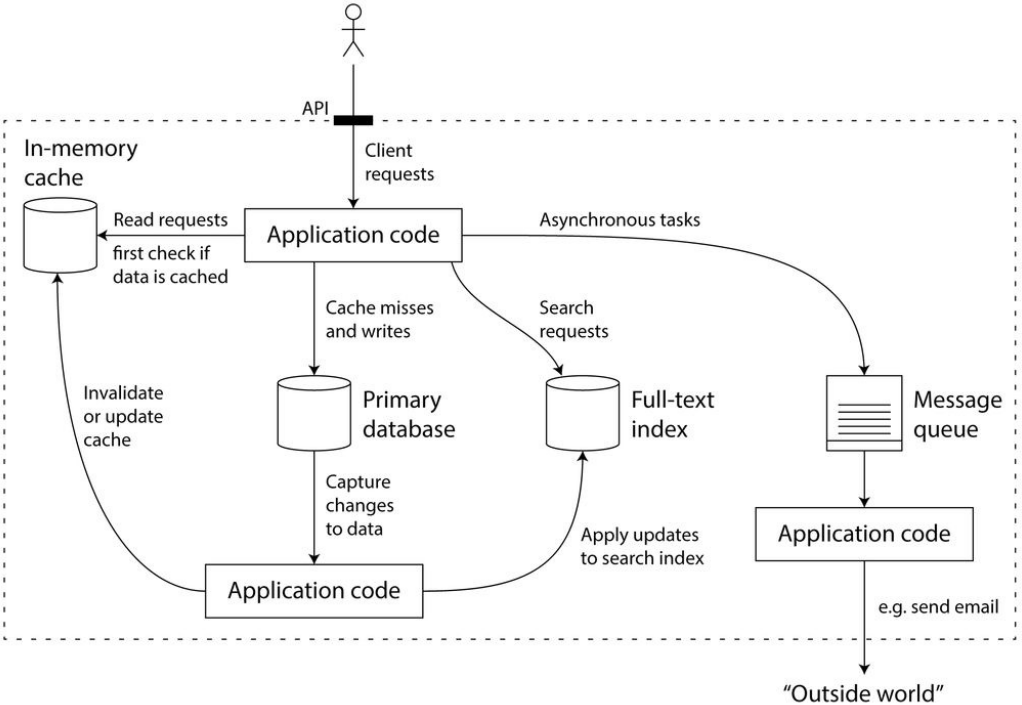
\includegraphics[scale=0.3]{1.png}
\end{center}

\subsection{Desafios que os Sistemas de Dados enfrentam}

\begin{flushleft}
  \item Como garantir que todos os dados se mantêm corretos e consistentes, mesmo quando, internamente, ocorreu algum erro? (ex: persistência de dados)
  \item Como fornecer boa performance para os clientes, mesmo quando partes do sistema estão degredadas?
  \item Como escalar o sistema para ser capaz de aguentar uma load intensiva de trabalho?
  \item Qual a aparência de uma boa API para o serviço?
\end{flushleft}

\subsection{Alguns Requisitos}

\begin{flushleft}
  \item \textbf{Fiabilidade -} O Sistema deve continuar a funcionar corretamente em caso de adversidades (ex: falhas de hardware, software ou mesmo humanas).
  \item \textbf{Escalabilidade -} O Sistema deve ser capaz de responder ao crescimento seja do volume de dados, do tráfego, ou mesmo da complexidade.
  \item \textbf{Manutenibilidade -} Deve ser possível que o Sistema sofra alterações ao longo do tempo por várias pessoas diferentes de forma produtiva.
\end{flushleft}

\pagebreak

\subsection{Bases de Dados}

\begin{flushleft}
  São definidas como um \uline{conjunto de dados relacionados entre si e a sua organização}.
  \vspace{2mm}
  Dividem-se em vários tipos, sendo atualmente os mais comuns: \textbf{Relacionais}, seguidas por
  \textbf{Documentais}, \textbf{Motores de busca}, \textbf{Chave-Valor}, entre outras. 
  \vspace{2mm}
  O controlo às bases de dados é realizado por \textbf{Sistemas de Gestão de Base de Dados} (\textbf{SGBD}
  ou DBMS em inglês). Estes fornecem funções que permitem a manipulação de grandes
  quantidades de informação.
\end{flushleft}

\section{NoSQL Databases - Key-Value Databases}

\begin{flushleft}
  \begin{enumerate}
    \item É o mais simples dos tipos NoSQL;
    \subitem Consiste apenas em chaves únicas e a um "bucket" que contêm qualquer tipo de dados que se pretenda;
    \item Pares chave-valor:
    \subitem \textbf{Chave}: (id, identificador, chave primária) Normalmente é uma String;
    \subitem \textbf{Valor}: Pode ser qualquer tipo de dados, texto, estrutura, imagem \dots;
    \item O conteúdo do valor ("bucket") pode ser, literalmente, qualquer coisa (mais comum é não estruturado ou semi-estruturado);
    \item Os "buckets" podem armazenar entradas pesadas, incluindo BLOBs (Basic Large Objects);
    \item Row based systems, utilizados para eficiência;
  \end{enumerate}
\end{flushleft}

\subsection{Vantagens}

\begin{enumerate}
  \item Tolerância a falhas elevada - sempre disponível;
  \item Schemaless, logo, muito flexível. oferece uma grande escalabilidade para mudar os requisitos dos dados;
  \item Eficiente a devolver dados de um objeto, com operações de disco minimas;
  \item Muito simples, rápido e fácil de dar deploy;
  \item Ótimo para escalabilidade horizontal (muitos servidores);
  \item Não necessita de queries SQL, indexes, triggers, sp's, views, \dots;
  \item Data ingest rates muito elevadas (muitos dados a entrar);
  \subitem Favorece: escreve uma vez, lê muitas vezes;
  \item Potente no "offline reporting" com data sets muito grandes;
  \item Existem formas avançadas de KVs que apresentam capacidades de document ou column oriented stores;
\end{enumerate}

\pagebreak

\subsection{Desvantagens}

\begin{enumerate}
  \item Não é apropriado para aplicação complexas;
  \item Não é eficiente a ataualizar records em que apenas parte do "bucket" é alterado;
  \item Não é eficiente em devolver informação limitada de records específicos (ex: returning only
  records of employees making between \$40K and \$60K); 
  \item Não é apropriado para queries complexas;
  \item Com o aumento do volume de dados, manter chaves únicas pode tornar-se um problema;
  \item Geralmente precisa de ler todos os records de um "bucket" ou talvez precise de contruir índices secundários;
\end{enumerate}

\subsection{Use Cases}

\begin{enumerate}
  \item Session data, user profiles, user preferences, shopping
  carts, \dots;
  \item Criar datasets que são raramente acessados mas crescem ao logo do tempo (Caching);
  \item Onde a performance de escrite é a prioridade;
\end{enumerate}

\subsection{Quando NÃO usar}

\begin{enumerate}
  \item Quando precisamos de ter relações entre entidades;
  \item Queries requerem acesso a conteúdos da parte dos valores;
  \item Set operations que envolvem múltiplos pares chave-valor;
\end{enumerate}

\subsection{Key Management}

\begin{flushleft}
  Como devem as chaves serem produzidas?

  \item \textbf{Manualy assigned keys} - Identificadores do mundo real (ex: e-mail, login names, \dots);
  \item  \textbf{Automatically generated keys} - Auto-incremente integers ou chaves mais complexas geradas por algotitmos;
\end{flushleft}


\pagebreak

\subsection{Query Patterns}

\begin{enumerate}
  \item Basic \textbf{CRUD} operations;
  \subitem Apenas quando a chave for dada;
  \subitem O conhecimento da chave é essencial;
  \subitem Ás vezes, pode ser até dificil para uma base de dados dar uma lista com todas as chaves;

  \item \textbf{No searching by value};
  \subitem Mas pode-se instruir à base de dados como dar parse aos valores, para fazer operações;

  \item \textbf{Batch / sequential processing}
  \subitem MapReduce;
\end{enumerate}

\subsection{Outras funcionalidades}

\begin{enumerate}
  \item Expiração de  pares chave-valor;
  \item Coleções de valores (We can store not only ordinary values, but also their
  collections such as ordered lists, unordered sets etc.);
  \item Links entre pares chave-valor (podem ser usados quando se usa queries);
\end{enumerate}

\subsection{Exemplos}

\begin{enumerate}
  \item \textbf{RiakKV}
  \item \textbf{Redis}
\end{enumerate}

(Ver slides 12-40)

\section{NoSQL Databases - Document Databases}

As bases de dados de documentos são bastante eficientes em cenários \textbf{one-to-many}.
Oferecem um esquema flexível (mesmo dentro das mesmas coleções (informação heterogénia)) e melhor performance
(devido ao armazenamento da informação junto à entidade a que esta se refere) que são
manipulados através de código simples.

\begin{flushleft}
  \textbf{Nota:} A flexibilidade permite que existam objetos na mesma coleção com atributos ligeiramente diferentes, sem necessidade
  de criarmos uma tabela para cada tipo de objeto.

  A localidade pode levar à duplicação de dados entre documentos.
\end{flushleft}

Um \textbf{documento} caracteriza-se por uma \textbf{string continua} codificada em JSON, XML,
ou outro formato binário estruturado.
É self-described (atributos são claros) e apresentam uma \textbf{estrutura em árvore}. São
identificados por um \textbf{id único}.

Geralmente, para manipular, é necessário carregá-lo por completo e para guardar as
alterações reescreve-lo na totalidade.

\begin{flushleft}
  \textbf{Nota:} A localidade só se torna uma vantagem se manipularmos porções grandes do documento.
\end{flushleft}

\pagebreak

Esta topologia não aplica a modelos \textbf{many-to-many}, pois não existem
operações de \textbf{join} de documentos. Deve também ser evitada quando a estrutura
do documento é demasiado instável (sempre a mudar).

\begin{flushleft}
  \textbf{Nota:} Não é desejável demasiada granularidade entre os documentos porque se todos apresentarem características
  diferentes não são relacionáveis e assim não fará sentido estarem na mesma coleção.
\end{flushleft}

No entanto, é a ideal para logging de eventos, sistemas de gestão de conteúdos,
blogues, web analytics, aplicações e-commerce \dots
Por ser a solução para alguns, mas não para todos os problemas, as bases de dados
relacionais começaram a incluir funcionalidades documentais e vice-versa.

\subsection{Exemplos}
  \begin{enumerate}
    \item \textbf{MongoDB}
    \item \textbf{CouchDB}
    \item \textbf{Couchbase}
  \end{enumerate}
  (Ver slides 11-51)

\section{Modelos de bases de dados}

Os modelos de dados com os quais os programas vão trabalhar têm um papel fundamental na
sua programação.
Têm um efeito enorme na forma como os programas são escritos e na forma como
nós pensamos sobre os problems que estamos a resolver. Todos os modelos de dados
têm formas diferentes de representar os dados e de os manipular.

\subsection{Bases de Dados Relacionais}

Este tipo de base de dados oferece vários benefícios (resolvendo a maior parte dos problemas com dados), entre os quais a \textbf{persistência} dos dados (ao guardar dados eles mantêm-se guardados),
a \textbf{integração} com várias aplicações (com a mesma DB) e a \textbf{atomicidade}, \textbf{consistência}, \textbf{isolamento} e \textbf{duranilidade}
oferecidas pelas \uline{transações} (ACID).

\subsubsection{Transactions - ACID Properties}

\begin{itemize}
  \item \textbf{Atomicidade} - Numa transação, ou todas as operações são executadas, ou nenhuma é;
  \item \textbf{Consistência} - É garantido que as restrições de integridade
  antes da transação se mantêm após esta;
  \item \textbf{Isolamento} - As alterações feitas na BD só são visíveis quando a transação termina.
  \item \textbf{Durabilidade} - Assim que commited, as alterações de uma transação persistem mesmo em caso de falhas.
  
  A durabilidade é garantida através das
transactions log, que permite a recunstrução das transações perdidas em caso
de falhas.
\end{itemize}

\pagebreak

\begin{center}
  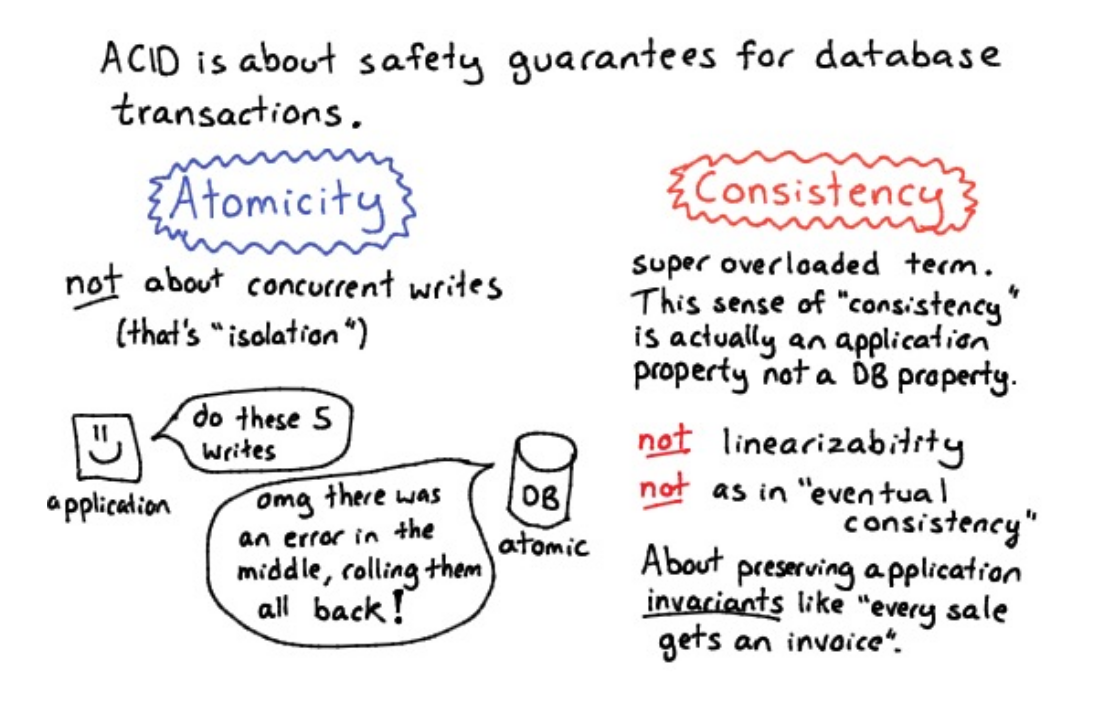
\includegraphics[scale=0.3]{2}
  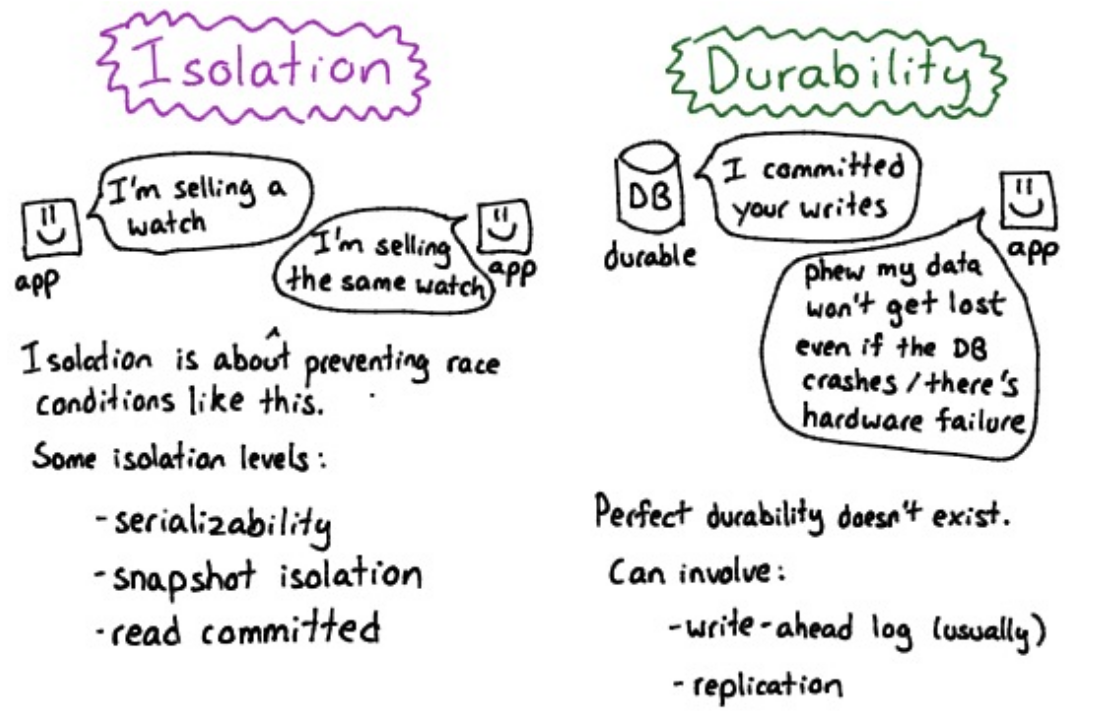
\includegraphics[scale=0.3]{3}
\end{center}

(Ver slides 7-8, história das bases de dados relacionais)

\pagebreak


\subsection{Current Trends and Issues}

\begin{flushleft}
  Algumas trends e issues motivaram à mudança nas tecnologias de armazenamento
de dados relacionais (em use cases e na tecnologia).

\textbf{Key Trends include:} Aumentar o volume de dados e tráfego. Ligação entre dados mais complexo.
\textbf{Key Issues include:} O problema $\rightarrow$ \textbf{impedance mismatch}.
\end{flushleft}

\subsection{Impedance Mismatch}

Nos últimos tempos, tem-se assistindo a um \textbf{aumento do volume de dados e tráfego}, a par da
redução do relacionamento entre eles, ou seja, \textbf{cada vez há mais dados não relacionados}.

Tem-se também verificado um conflito entre os \uline{princípios de engenharia de
software}, onde o
paradigma é \uline{orientado a objetos} e os princípios relacionais baseados em \uline{modelos
matemáticos}. Este problema é designado por \textbf{Impedance} (oposição que um circuito elétrico faz à passagem de corrente elétrica quando é submetido a tensão)
\textbf{Mismatch} (Disparidade, incompatibilidade).

Atualmente, este verifica-se nas estruturas isoladas, que violam os princípios da \textbf{normalização}.
Para armazenar informação persistentemente em programas modernos, uma única
estrutura lógica tem de ser separada (\textbf{normalização}).

\subsubsection{Exemplo}

Vários objetos que representem funcionários numa empresa. Cada funcionário terá o seu departamento,
mas vários funcionários podem trabalhar no mesmo departamento. Se a base de dados refletir o paradigma orientado a
objetos, iremos ter uma repetição dos departamentos nos vários funcionários e base de dados não estará normalizada!

No entanto, fazer múltiplos selects e joins para construir uma entidade às vezes não é a melhor opção.

\begin{center}
  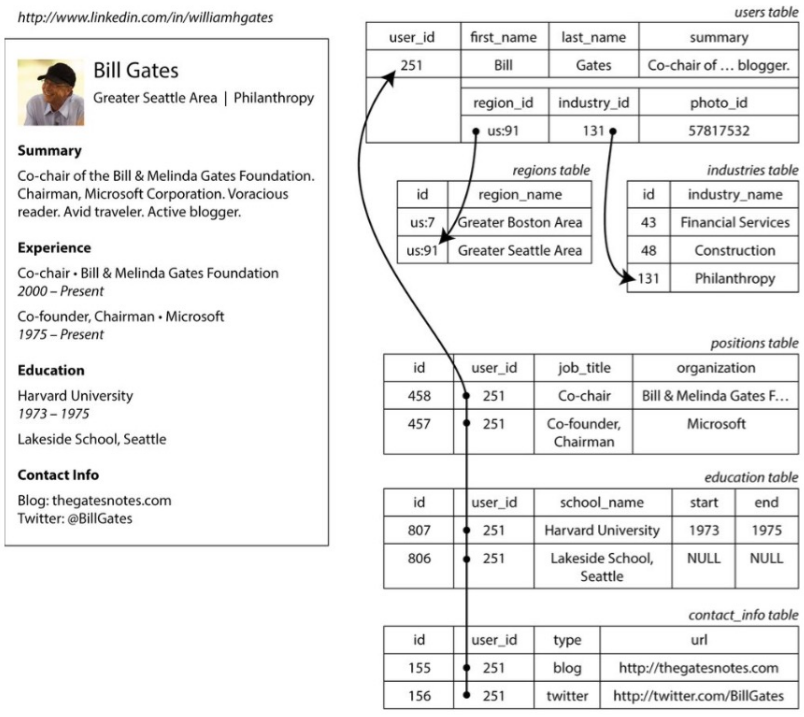
\includegraphics[scale=0.3]{4}
\end{center}

\pagebreak

\subsubsection{One-to-Many relations}

\begin{center}
  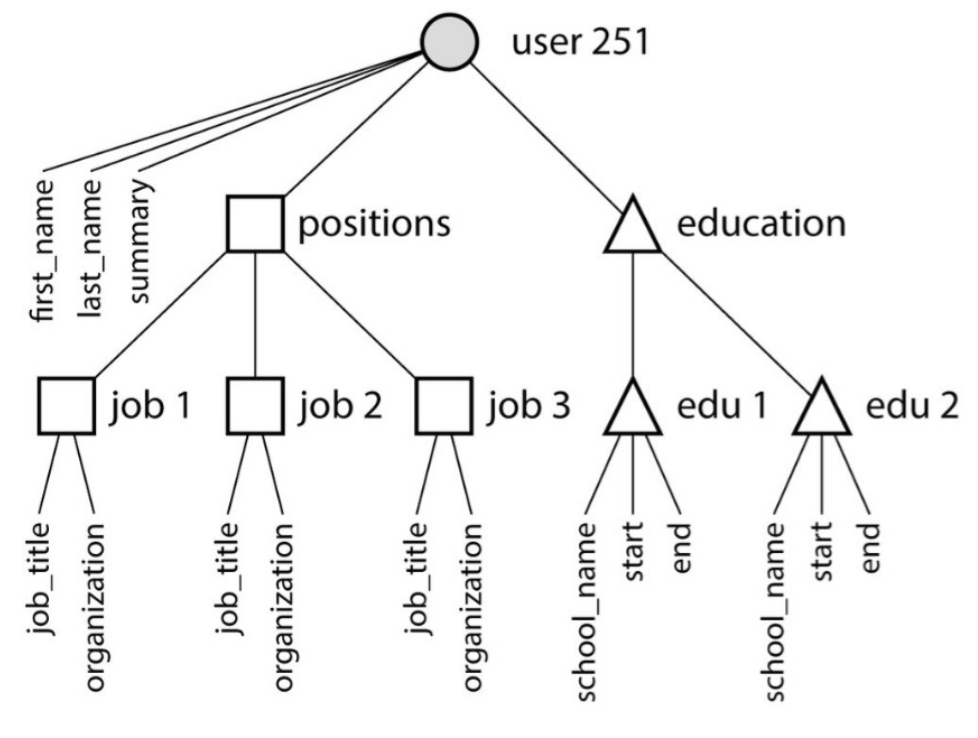
\includegraphics[scale=0.2]{5}
\end{center}

\subsection{Normalização}

Tem o objetivo de \textbf{reduzir a redundância dos dados}.
Em DB's este reflete-se na \uline{utilização de IDs} para identificar entidades,
oferecendo uma \textbf{consistência de utilização}, ao mesmo tempo que
\textbf{previne ambiguidades}, caso hajam entidades semelhantes (ex: com o mesmo nome),
\textbf{facilita alterações} das entidades, uma vez que a sua informação está armazenada
numa única tabela, motivo pelo qual também \textbf{facilita a tradução}.

\begin{flushleft}
  \textbf{Nota:} Uma base de dados que verifica estas características diz-se \textbf{normalizada}.
  Uma base de dados na qual as entidades como região e industria estão referidas
  por ID diz-se \textbf{normalizada}.

  No entanto, uma basde de dados que duplica nomes e propriedades de entidades
  em cada documento diz-se \textbf{desnormalizada}.
\end{flushleft}

\subsubsection{Many-to-Many relationships}

\begin{center}
  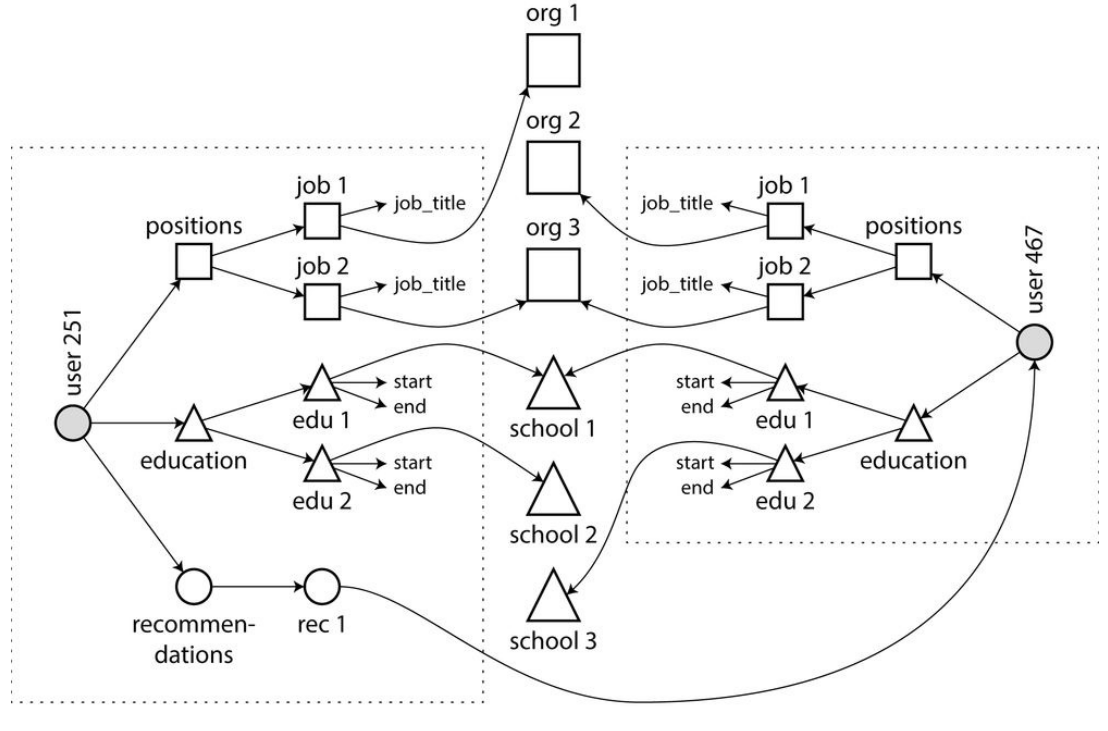
\includegraphics[scale=0.25]{6}
\end{center}

\pagebreak

\subsection{Responder ao aumento do volume de dados}

We are creating, storing, processing more data than ever before!

\vspace{3mm}
Existem duas abordagens possíveis:
\begin{itemize}
  \item Contruir bases de dados mauores;
  \item Criar um grupo de máquinas mais pequenas que se complementam;
\end{itemize}

\begin{enumerate}
  \item A primeira abordagem tem alguns problemas, uma vez que o \textbf{custo}
  de duplicar a capacidade de uma DB é geralmente mais do dobro do custo de uma
  DB "normal" e mesmo com recursos financeiros, há \textbf{limitações físicas} e de
  engenharia à sua capacidade;
  
  \item A segunda, apesar de mais exequível, tem também alguns defeitos, uma vez
  que por ser uma solução \textbf{barata}, pode refletir-se em \textbf{menos
  fiabilidade}. É ainda nexessário a integração com um DBMS compatível com
  a tipologia.
\end{enumerate}

Os Sistemas de Gestão de Bases de Dados (DBMS) têm alguma \textbf{dificuldade em gerir a escalabilidade
horizontal} (distribuição da BD).

\subsection{O movimento NoSQL}

Este movimento, cujo acrónimo significa
\textbf{Not only SQL}, pretende promover a utilização de bases
de dados não relacionais (SQL). Tem por base vários princípios.

\begin{enumerate}
  \item \textbf{Não é relacional} - Podem ser mas não são boas nisso;
  \item \textbf{API simples} - Sem necessidade de realizar \uline{join};
  \item \textbf{Teorema BASE \& CAP} - Viola os princípios ACID;
  \item \textbf{Schema-free} - Esquema implícito e gerido pela aplicação (sem verificações do lado da DB);
  \item \textbf{Distribuídas} - Algumas mais do que outras;
  \item \textbf{Open-source} - Mostly;
\end{enumerate}

\subsubsection{Transações BASE}

Este acrónimo nasceu em oposição aos princípios ACID, principalmente
em resposta às limitações de consistência que um cenário de um sistema
distribuído impõe.

\begin{itemize}
  \item \textbf{\uline{B}asic \uline{A}vailability} - A DB funciona a maior parte do tempo;
  \item \textbf{\uline{S}oft-state} - As manipulações dos dados não têm de ser write-consistent, nem
  diferentes réplicas têm de ser mutualmente consistentes o tempo todo.
  Escritas num nó da base de dados não têm de ser escritas garantidamente em simultâneo nos restantes nós;
  \item \textbf{\uline{E}ventual consistency} - O armazenamento de dados eventualmente torna-se consistente, em algum ponto
  (e.g. lazily at read time);
\end{itemize}

As bases de dados NoSQL caracterizam-se então por ser \textbf{otimistas} e \textbf{simples}, o que torna a
base de dados mais \textbf{rápida}, \textbf{disponibilidade em primeiro lugar}, \textbf{best effort} e \textbf{appoximate answers OK}.

\pagebreak

\subsubsection{Teorema CAP (Brewer's)}

Este teorema diz que um sistema distribuído só pode apresentar duas de três características:

\begin{itemize}
  \item \textbf{\uline{C}onsistent} - Escritas atómicas em toda a DB em simultâneo;
  \item \textbf{\uline{A}vailable} - A DB responde sempre a pedidos;
  \item \textbf{\uline{P}artition Tolerant} - O sistema consegue funcionar mesmo que um nó deixe de responder;
\end{itemize}

\begin{center}
  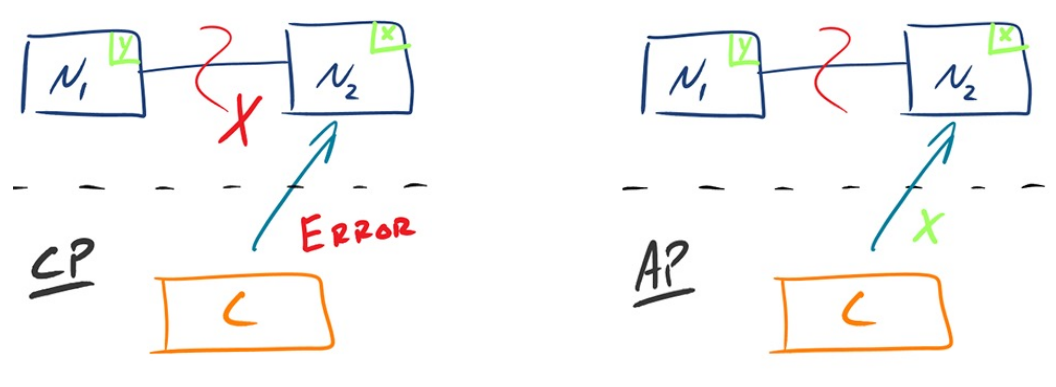
\includegraphics[scale=0.3]{7}
\end{center}

\begin{flushleft}
  \begin{enumerate}
    \item No primeiro temos uma base de dados que implementa a consistência e a tolerância a falhas.
    Quando um cliente faz um pedido de consulta de um valor, caso o nó não consiga contactar os restantes de forma a
    confirmar que todos têm o mesmo valor, retorna uma mensagem de erro.
    \item No segundo temos a disponibilidade e tolerância a falhas. Neste caso, mesmo com uma falha de comunicação entre
    os nós, o nó contactado pelo cliente vai responder com o valor pedido, mesmo que este não seja o mai atual.
  \end{enumerate}
\end{flushleft}

\begin{center}
  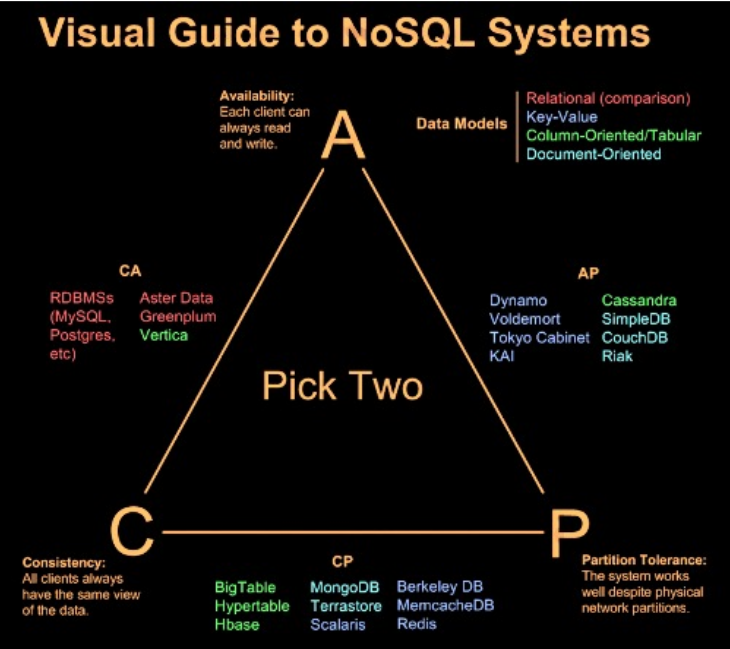
\includegraphics[scale=0.3]{8}
\end{center}

\pagebreak

\subsection{Tipos de Bases de Dados NoSQL}

\begin{flushleft}
  Existem vários tipos de bases de dados NoSQL. Core types:
  \begin{itemize}
    \item \textbf{Key-value stores}
    \item \textbf{Document stores}
    \item \textbf{Column stores}
    \item \textbf{Graph databases}
  \end{itemize}

  Non-core types:
  \begin{itemize}
    \item \textbf{Object databases}
    \item \textbf{Native XML databases}
    \item \textbf{RDF stores}
    \item \textbf{\dots}
  \end{itemize}
\end{flushleft}

\subsubsection{Key-value Databases}

Esta base de dados está focada em \textbf{armazanamento chave-valor}. É a mais simples
e funciona como uma simples hash table, tabela de dispersão (mapping).

\begin{flushleft}
  \textbf{Chave} - Identificador (chave primária) único, normalmente uma string;
  
  \textbf{Valor} - Pode assumir uma variedade de tipos, desde texto a estruturas de dados, \dots;
\end{flushleft}

As \uline{operações} são realizadas \uline{sobre um valor} de uma determinada chave.

A sua \textbf{simplicidade} permite uma boa \textbf{performance} e facilidade na \textbf{escalabilidade}. No entanto,
\uline{não permite} a realização de
queries complexos nem o armazenamento de dados complexos.
Usadas para perfis de utilizadores, informações de sessão, carrinhos de compras, preferências do utilizado, \dots

Tipicamente armazenam \uline{dados não persistentes}. \uline{Não permitem relações entre entidades}.
Não usar quando existem relações entre entidades, ou quando as queries pretendem
ter acesso aos valor.

\subsubsection{Document Databases}

O modelo de dados é uma estrutura complexa (tipicamente JSON ou XML), \textbf{self-describing},
uma vez que o nome dos atributos se descreve a si próprio, organizadas
numa \textbf{estrutura hierárquica} e onde cada documento tem um \textbf{identificador único}.

Pertmitem \uline{queries} sobre vários documentos, não só pela sua chave (id),
mas também pelo seu valor. É possível contruir índices, nos query patterns
podemos criar, atualizar e remover documentos, bem como é possível fazer
pesquisa usando queries complexas.

Quando comparadas com as bases de dados chave-valor, estas são uma evolução,
em que o valor é examinavél.

\begin{center}
  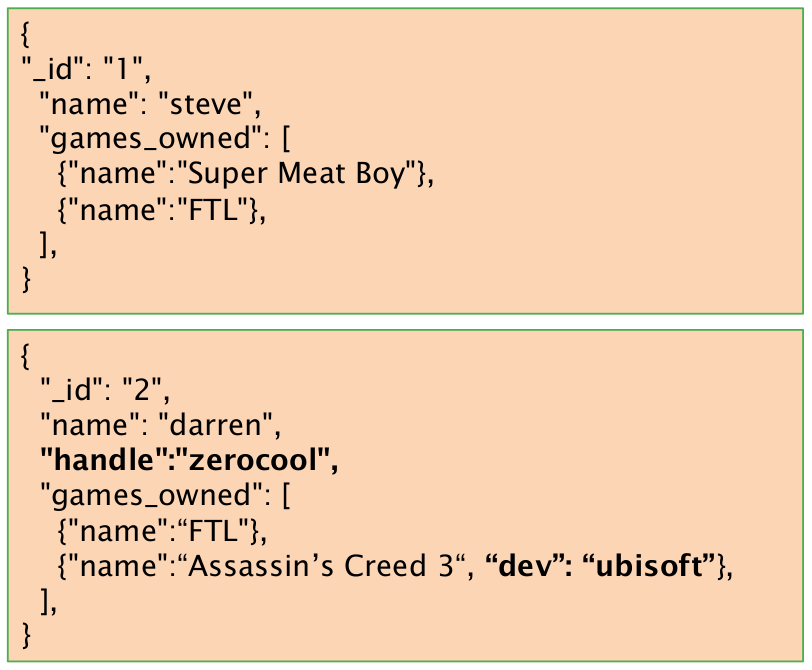
\includegraphics[scale=0.2]{9}
\end{center}

\begin{flushleft}
  \textbf{Usar:} Log de eventos, blogs, sistemas de gestão de conteúdos,
  web analytics, aplicações e-commerce, \dots
  \textbf{Documentos estruturados com um schema semelhante}.

  \textbf{Não usar:} Operações de \textbf{set} que envolva múltiplos documentos,
  onde o design da estrutura do documento esteja sempre a mudar e
  em relações \textbf{many-to-many}.
\end{flushleft}

\subsubsection{Column Databases}

\begin{flushleft}
  \textbf{Data Model:}
  \begin{itemize}
    \item \textbf{Familia de Colunas (Table)}
    \begin{itemize}
      \item Table é uma coleção de rows similares (mas não necessariamente identicas);
    \end{itemize}
    \item \textbf{Row}
    \begin{itemize}
      \item Coleção de colunas - deve compactar um grupo de dados a ser acedidos juntos;
      \item Associado a uma chave única de row (row key);
    \end{itemize}
    \item \textbf{Column}
    \begin{itemize}
      \item Consiste no nome da coluna, valor da coluna (possivelmente outros metadados)
      \item Valores escalares, sets flat, listas ou maps;
    \end{itemize}
  \end{itemize}

  \textbf{Query Patterns:}
  \begin{itemize}
    \item Criar, atualizar ou remover row de uma dada familia de colunas;
    \item Selecionar rows de acordo com a row key ou outras condições simples;
  \end{itemize}

  \textbf{Use Cases:}
  \begin{itemize}
    \item Event logging, content management systems, blogs, \dots
    \item Basicamente tudo o que for structured flat data com um schema parecido
    \item Batch processing via MapReduce;
  \end{itemize}

  \pagebreak

  \textbf{Quando NÃO usar:}
  \begin{itemize}
    \item Precisamos de ACID transactions;
    \item Queries complexas (aggregation, joins, \dots);
    \item Prototipos iniciais (quando o design da bd ainda está sujeita a mudanças)
  \end{itemize}
\end{flushleft}

\subsubsection{Graph Databases}

\begin{flushleft}
  \textbf{Data Model:}
  \begin{itemize}
    \item Foco na modelação da estrutura e propriedade dos grafos;
    \item Grafos podem ser ou não direcionados;
    \item Grafos são coleções de:
    \begin{itemize}
      \item Nós (vertices) para entidades do mundo real;
      \item Relações (edges) entre estes nós;
    \end{itemize}
    \item Ambos os nós e relações podem ter propriedades;
  \end{itemize}

  \textbf{Query Patterns:}
  \begin{itemize}
    \item Criar, atualizar ou remover nós/relações do grafo:
    \begin{itemize}
      \item Algoritmos de Grafos
      \item General Graph Traversal
      \item Sub-Graph ou Super-Graph Queries
      \item Similarity based Queries
    \end{itemize}
  \end{itemize}

  \textbf{Use Cases:}
  \begin{itemize}
    \item Social networks, routing, dispatch, location based services, \dots
  \end{itemize}

  \textbf{Quando NÃO usar:}
  \begin{itemize}
    \item Quando operações extensivas de batch são necessárias (múltiplos nós/relações
    são afetadas);
    \item Vamos dar store de grafos demasiado grandes (a distribuição de grafos ou até mesmo impossível);
  \end{itemize}
\end{flushleft}

\pagebreak

\subsubsection{Native XML Databases}

\begin{flushleft}
  \textbf{Data Model:}
  \begin{itemize}
    \item Documentos XML;
    \item Estrutura em árvore com nested elements, atributos e valores de texto;
    \item Documentos organizados em coleções;
  \end{itemize}

  \textbf{Query Languages:}
  \begin{itemize}
    \item Xpath (XML Path Language);
    \item XQuery (XML Query Language);
    \item XSLT (Extensible Stylesheet Language Transformations);
  \end{itemize}
\end{flushleft}

\subsubsection{RDF Databases}

\begin{flushleft}
  \begin{itemize}
    \item RDF Triples
    \begin{itemize}
      \item Subject, Predicate, Object;
      \item Cada Triple representa uma statement sobre uma entidade do mundo real;
    \end{itemize}
    \item Triples podem sser vistas em grafos
    \begin{itemize}
      \item Vertices representam os subjects e objects;
      \item Edges correspondem diretamente às statements individuais;
    \end{itemize}
  \end{itemize}

  \textbf{Query Languages:}
  \begin{itemize}
    \item SPARQL (SPARQL Protocol and RDF Query Language);
  \end{itemize}
\end{flushleft}

\subsubsection{Databases and data connectivity}

\begin{center}
  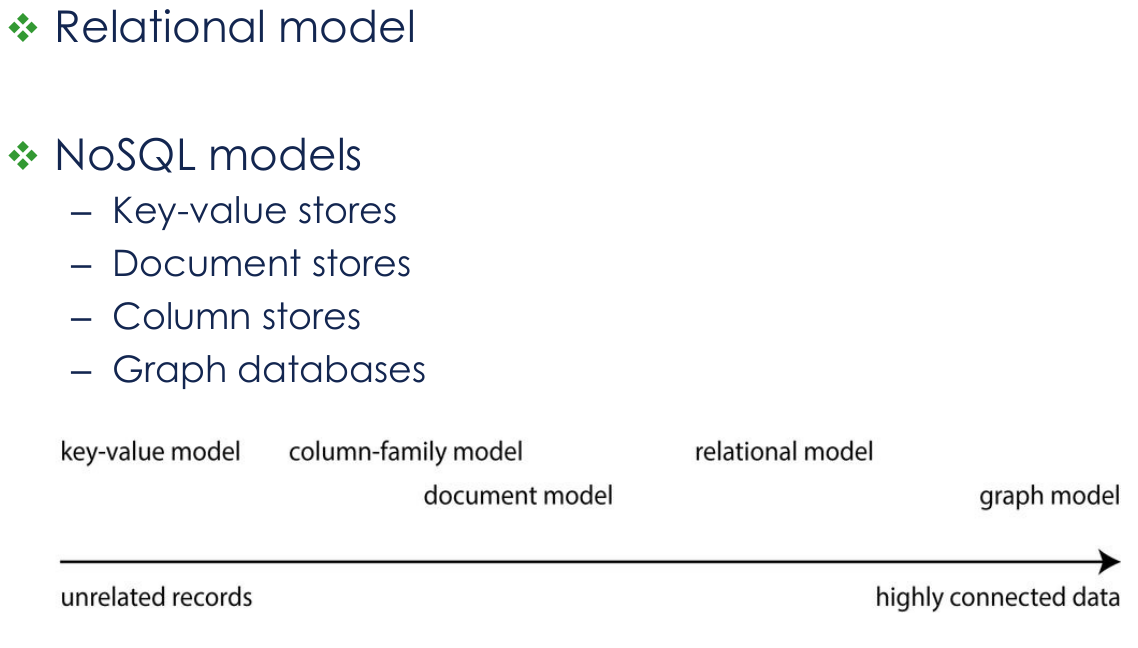
\includegraphics[scale=0.25]{41}
\end{center}

\pagebreak

\subsubsection{Considerações Finais}

As NoSQL DBs \textbf{NÃO} são o fim das bases de dados relacionais.
Estas continuam a ser preferiveis para 90\% dos projetos, para além do facto
das pessoas estarem mais familiarizadas, serem mais estáveis, terem mais
fearures e mais documentação e suporte disponível.

Mesmo assim devemos considerar diferentes modelos e sistemas de bases de dados.

\vspace{2mm}

\begin{flushleft}
  \textbf{Persistência Poliglota} - Uso de diferentes data stores em diferentes circunstâncias.
\end{flushleft}






\pagebreak
\section{NoSQL Databases - Column Databases}

A ideia geral é que vamos \textbf{armazenar e processar dados por coluna} (column) em vez de por linha
(row). Geralmente tem origem em queries agregadores de dados, que permitem gerar
dados suscetíveis de serem analisados para fins \textbf{estatísticos} ou para \textbf{business intelligence}.

Visa então os \uline{serviços acima da utilização do armazenamento}, permitindo \textbf{processamento paralelo}
e consequentemente a construção de \textbf{aplicações de alto desempenho}.

A falta de normalização faz com que os dados sejam esparsos e que hajam bastantes campos
nulos. É descrita como: “sparse, distributed, persistent
multidimensional sorted map”.

\begin{center}
  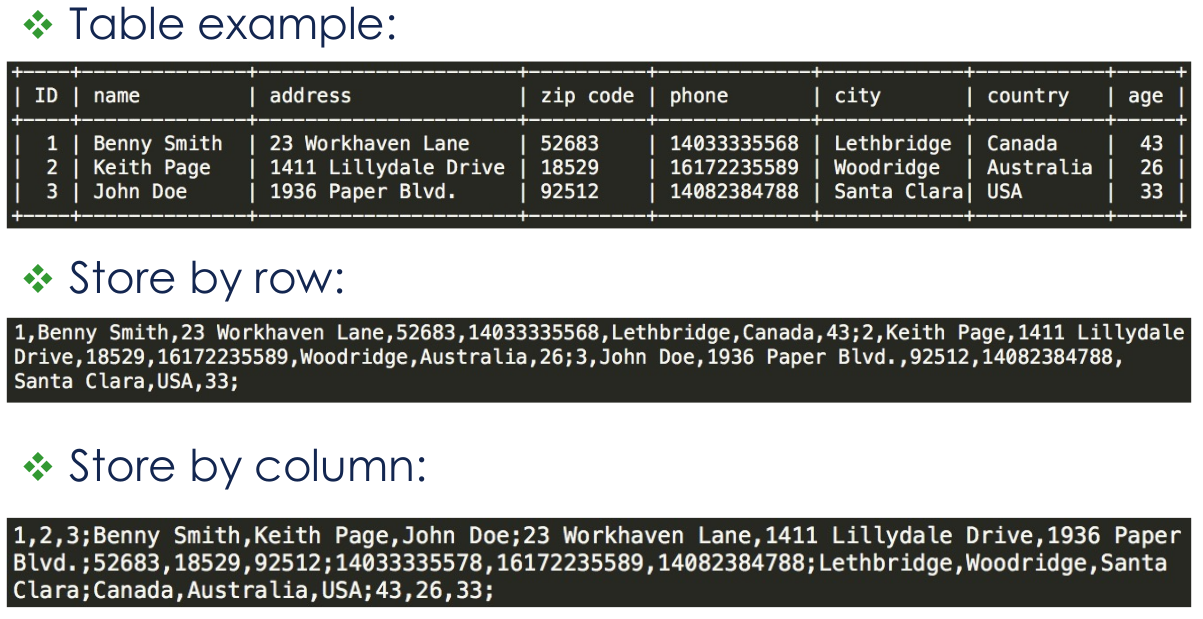
\includegraphics[scale=0.3]{10}
  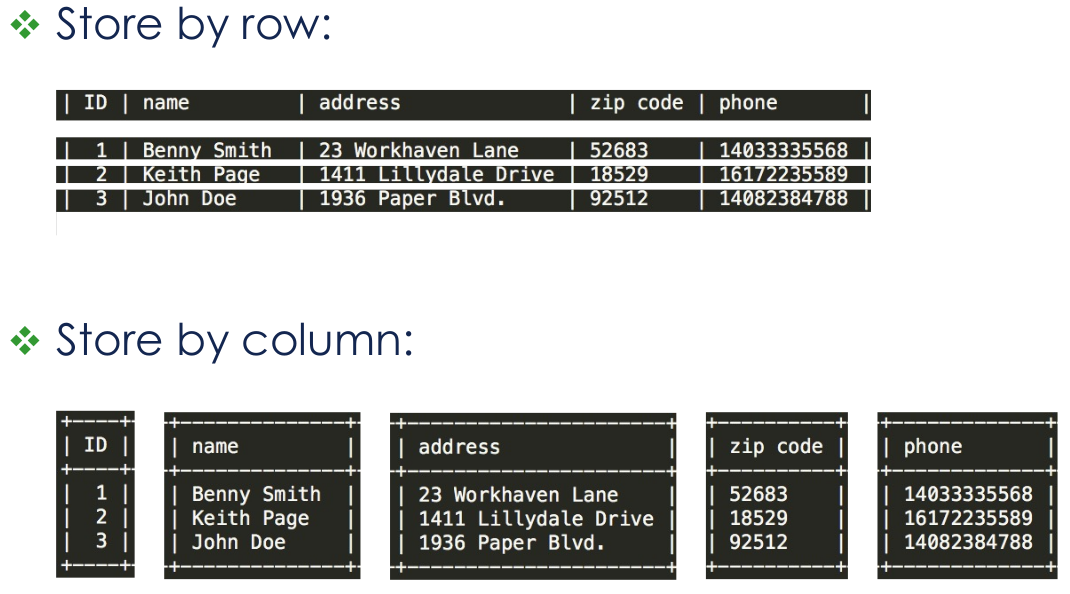
\includegraphics[scale=0.3]{11}
\end{center}

\pagebreak

\subsection{Vantagens}
É vantajoso em cenários em que são feitos \textbf{queries com poucas colunas sobre
grandes volumes de dados}. Destaca-se ainda a maior \textbf{facilidade de compressão} por colunas,
uma vez que estes dados neste domínio tendem a estar mais relacionados.

\subsubsection{Explicado}
Torna algumas queries mesmo muito rápidas:
\begin{itemize}
  \item Aggregation queries;
  \item Funções sobre fields (ex: average salary);
\end{itemize}
Melhor compressão de dados:
\begin{itemize}
  \item Ao correr o algoritmo em cada coluna (dados similares);
  \item Mais notável quando começamos a ter datasets grandes;
\end{itemize}

\subsection{Desvantagens}
Possui algumas desvantagens, como o \textbf{carregamento incremental de dados}, o uso de \textbf{OLTP}
(OnLine Transaction Processing), ou a realização de \textbf{queries a linhas} (dados individuais).

\subsubsection{Explicado}

Aggregation é bom, mas algumas aplicações precisam de ser capazes de mostrar dados para
cada \uline{individual record}. BDs colunares são geralmente não muito boas para esses tipos de queries.
Escrever novos dados pode demorar tempo, inserir um novo record numa row oriented database é uma simples
write operation. Fazer update de muitos values numa column db pode demorar muito tempo.

\vspace{2mm}

O \textbf{carregamento incremental} de dados caracteriza-se por atualizações constantes. É uma desvantagem porque a cada
inserção têm de se editar todos os ficheiros de todas as colunas, pelo que este processo geralmente é realizado
periodicamente e para grandes volumes de dados em simultâneo.

\vspace{2mm}

Contrariamente às bases de dados relacionais, são \textbf{orientadas aos serviços}
e não aos dados.

\vspace{2mm}

Nasceu com o projeto \textbf{Bigtable} da Google, que serviu de inspiração
aos restantes SGBD's colunares. Foi criado em resposta ao problema de greração
de índices para o seu motor de busca, que levava demasiado tempo.
Atualmente é utilizado também no Gmail e Google Maps.

\pagebreak

\subsection{Modelo de Dados}

\begin{flushleft}
  \textbf{Familia de colunas (tabela)} - Uma tabela é uma coleção de linhas semelhantes
  (não necessariamente idênticas).

  \textbf{Linha} - Uma linha é um conjunto de colunas (deve abranger um grupo de dados
  que é acessado em conjunto).
  Associado com uma chave de linha (row key) única.

  \textbf{Coluna} - Uma coluna consiste num nome de coluna (column name)
  e um valor de coluna (column value), possivelmente outros records de metadados.
  Valores escalares, mas também sets, listas e mapas.
\end{flushleft}

\subsection{Casos de Uso}

As bases de dados orientadas a colunas são utilizadas para o armazenamento de
dados estrutrados com um esquema similar, como log de eventos, sistemas de
gestão de conteúdo, blogs, \dots

Processamento de dados em batch via MapReduce.

\vspace{2mm}

Não é recomendado a utilização deste tipo de bases de dados quando
\textbf{transições ACID} (atomicidade, consistência, isolamento, durabilidade) são necessárias,
quando é necessário usar \textbf{queries complexas} como joins, nem \textbf{prototipagem} (o design da BD pode mudar), uma vez que a
sua orientação ao serviço, a torna altamente dependente dos seus requisitos.

\subsection{Tecnologias Representativas}

\begin{center}
  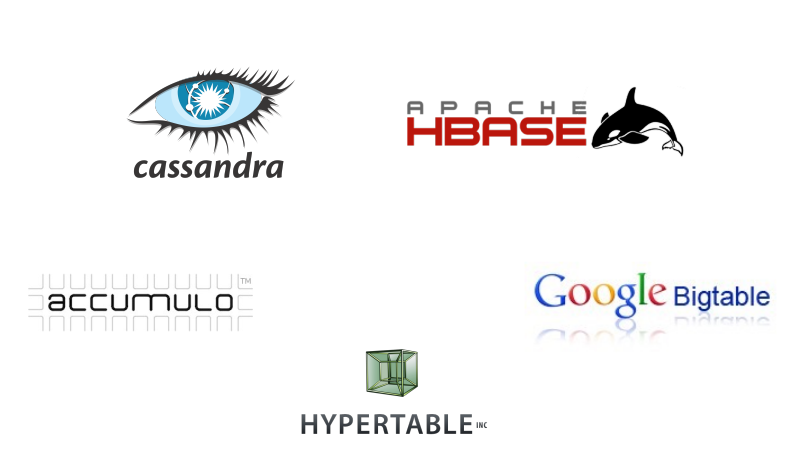
\includegraphics[scale=0.3]{12}
\end{center}

\textbf{Bigtable} é a inspiração para as datastores orientadas a colunas.
Bases de daods influenciadas pela Bigtable:
\begin{itemize}
  \item \textbf{HBase}
  \item \textbf{HyperTable}
\end{itemize}

\textbf{Cassandra} é uma extensão da Bigtable com aspetos do Dynamo da Amazon.

\pagebreak

\subsection{Apache Cassandra}

\subsubsection{Introdução}

É uma Cross Plataform, \textbf{open-source} Column Database, cujas features incluem
\textbf{alta disponibilidade}, \textbf{escalabilidade linear},
\textbf{fragmentação}, \textbf{replicação P2P configuravél},
\textbf{consistência tunable} e \textbf{suporte para MapReduce}.

Atualmente é o sistema de bases de dados orientado a colunas mais utilizado.
Foi inicialmente desenvolvido pelo Facebook (2008) mas atualmente está sob gestão da
fundação para o software Apache.

É ainda de destacar o alto desempenho na escrita, sem prejudicar a eficiência das leituras.
Por exemplo: Para dados com uma dimensão superior a 50GB, as escritas e leituras levariam cerca de 300ms. A Cassandra oferece
leituras a 0,12ms e escritas a 0,15ms.

\subsubsection{Motivação}
\begin{itemize}
  \item High availability;
  \item High write throughput, sem sacrificar read efficiency;
  \item Fault tolerance;
  \item High and incremental scalability;
  \item Reliablility at massive scale;
\end{itemize}

\subsubsection{Topologia do Sistema}

\begin{center}
  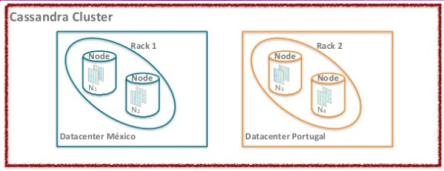
\includegraphics[scale=0.3]{13}
\end{center}

\begin{flushleft}
  \textbf{Node} - É a unidade base destes sistemas, são máquinas
  onde a Cassandra está em execução.

  \vspace{2mm}

  \textbf{Data Center} - Os nós são agrupados em data centers.
  Conjunto de nós relacionados entre si, que fazem \uline{replicação dos dados}
  de forma a garantir a \textbf{tolerância a falhas}.

  \vspace{2mm}

  \textbf{Cluster} - Conjunto de data centers sobre os quais são escritos
  os mesmo dados.
\end{flushleft}

\pagebreak

\subsubsection{Arquitetura do Sistema}

\begin{flushleft}
  \textbf{Cluster Membership} - Como é que os nodes são adicionados ou
  apagados de um cluster.

  \vspace{2mm}

  \textbf{Partitioning}
  \begin{itemize}
    \item Como é que os dados são particionados pelos nodes;
    \item Nodes são logicamente estruturados numa \textbf{Ring Topology};
    \item Hashed Values e Keys associados a Data Partitions são usadas para
    lhes dar assign a um node no ring.
  \end{itemize}

  \vspace{2mm}

  \textbf{Replication}
  \begin{itemize}
    \item Como é que os dados são duplicados pelos nós;
    \item Cada DataItem é replicado por N (replication factor) Nodes.
  \end{itemize}
\end{flushleft}

\subsubsection{Topologia do Sistema}

\begin{center}
  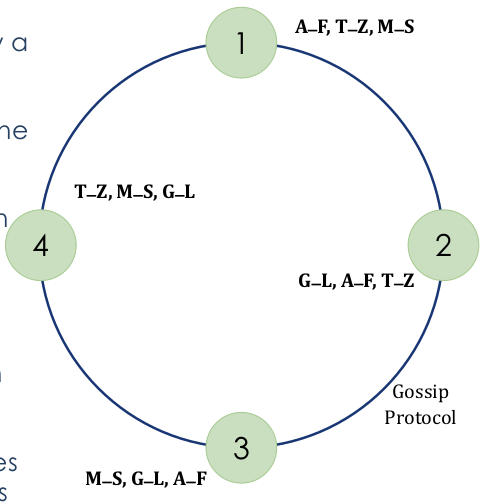
\includegraphics[scale=0.3]{14}
\end{center}

\begin{itemize}
  \item Cluster Data é gerida por um Ring of Nodes;
  \item Cada Node tem parte da BD;
  \item Rows são distribuidas baseadas na primary key;
  \item Rows são distribuidas baseadas na primary key (Row Lookups são rápidos);
  \item Múltiplos nodes tem os mesmos dados, para garantir availability e durability;
  \item Não há nenhum master node - Todos os nodes podem realizar todas as operações;
\end{itemize}

\pagebreak

\subsubsection{Modelo de dados}
\subsubsection*{Keyspaces $>$ Tables $>$ Rows $>$ Columns}

\begin{flushleft}
  \textbf{Keyspace:}
  \begin{itemize}
    \item É um \textbf{namespace} que define data replication nos nodes;
    \item Um cluster contém \textbf{um keyspace por node};
  \end{itemize}

  \vspace{2mm}

  \textbf{Table (Column Family):}
  \begin{itemize}
    \item Coleção de rows (parecidas);
    \item Multi-Dimensional Map indexado por chave (row key);
    \item Tables Schema tem de ser especificado mas pode ser modificado;
    \item 2 tipos: Simple ou Super (nested Column Families);
  \end{itemize}

  \vspace{2mm}
  
  \textbf{Row:}
  \begin{itemize}
    \item Coleção de colunas;
    \item Rows numa table não precisam de ter as mesmas colunas
    \item Cada Row É \textbf{uniquely identified} por uma \textbf{primary key};
  \end{itemize}

  \vspace{2mm}

  \textbf{Column:}
  \begin{itemize}
    \item Name-Value Pair + Dados Adicionais;
  \end{itemize}
\end{flushleft}

\begin{figure}[!h]
  \centering
  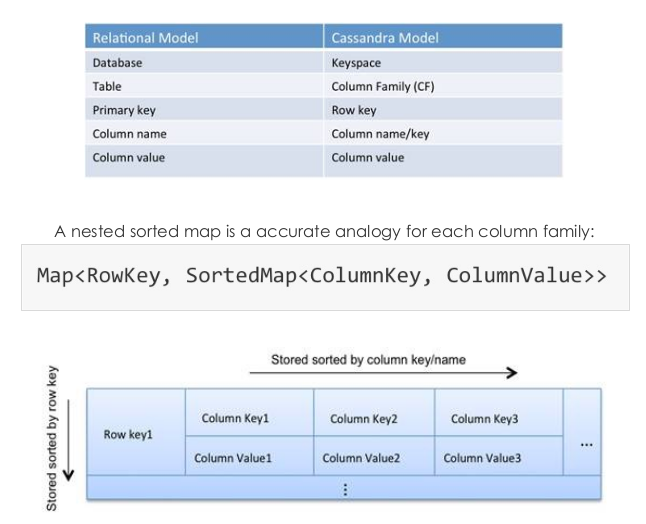
\includegraphics[scale=0.3]{15}
  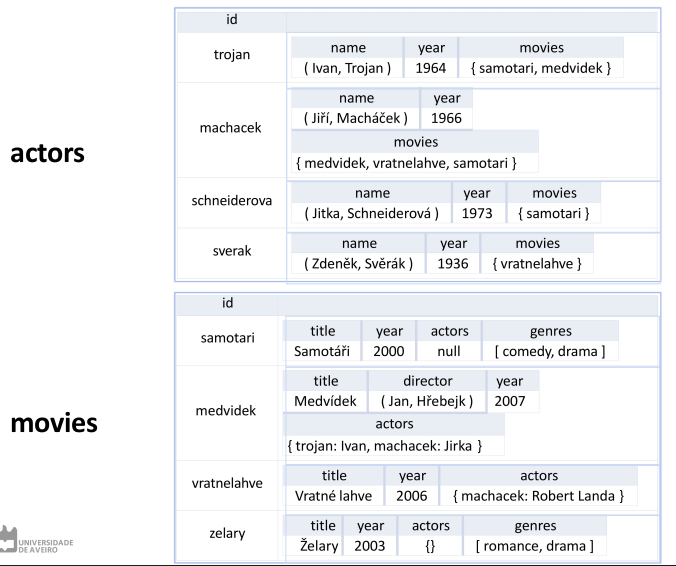
\includegraphics[scale=0.3]{16}
  \caption{Exemplo de um Data Model}
\end{figure}

\pagebreak

\subsubsection{Cassandra vs Relational Example}

\begin{figure}[!h]
  \centering
  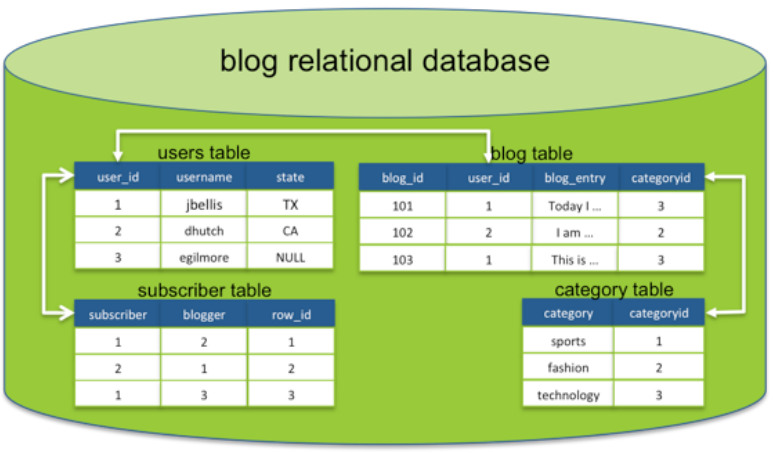
\includegraphics[scale=0.25]{17}
  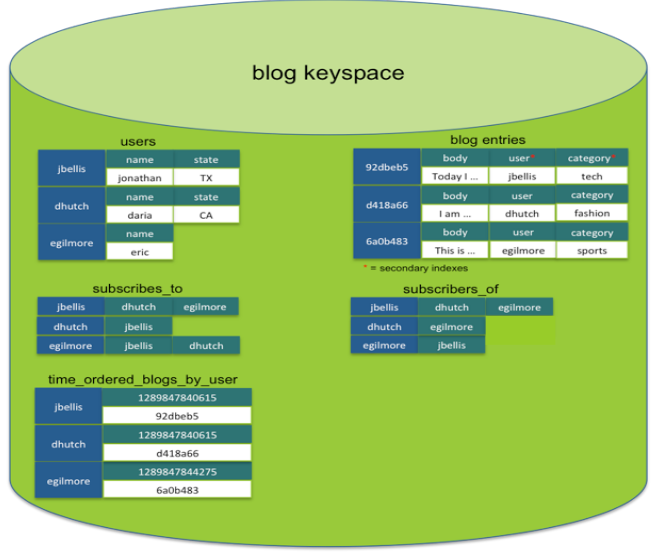
\includegraphics[scale=0.25]{18}
\end{figure}

\subsubsection{Column Values}
\begin{flushleft}
  Os value types aceites pelas colunas são:
  \begin{itemize}
    \item \textbf{Empty Value}
    \begin{itemize}
      \item Null
    \end{itemize}
    \item \textbf{Atomic Value}
    \begin{itemize}
      \item \textbf{Native Data Types} (Text, Integers, Dates, \dots)
      \item \textbf{Tuples} (Tuplo de fields anonimos, cada um com o seu Type
      (podendo cada membro do tuplo ter um type diferente))
      \item \textbf{User Defined Types (UDT)} (Set de named fields para cada type)
    \end{itemize}
    \item \textbf{Collections}
    \begin{itemize}
      \item \textbf{Lists}, \textbf{Sets} e \textbf{Maps} (Nested Tuples, UDTs ou collections são
      permitidos mas apenas um Forzen Mode (elementos são serializados quando
      são guardados))
    \end{itemize}
  \end{itemize}
\end{flushleft}

\subsubsection{Data Model - Dados adicionais}

Associados a cada coluna no caso dos atomic values ou qualquer element de uma
collection.

\begin{flushleft}
  \textbf{Time to Live (TTL):} Após um certo tempo (segundos) um dado value é automaticamente apagado;

  \vspace{2mm}

  \textbf{Timestamp:} Timestamp de quando a última modificação foi feita. Fornecido
  automaticamente ou manualmente;
\end{flushleft}

Ambos estes elementos podem ser queried mas não no caso de collections e dos seus
elementos.

\pagebreak

\subsubsection{Cassandra API}

\begin{flushleft}
  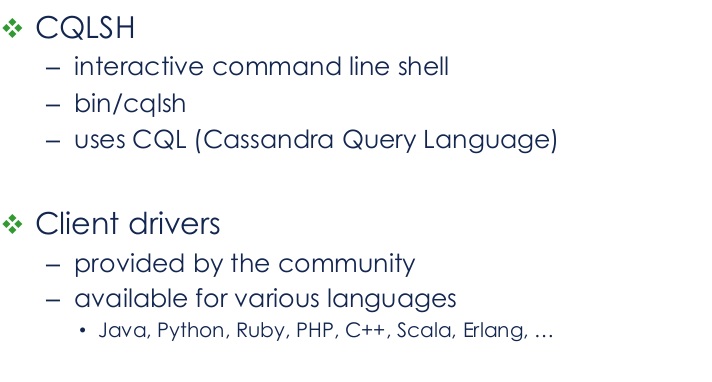
\includegraphics[scale=0.3]{19}
\end{flushleft}

\subsection{Cassandra Query Language (CQL)}

Declarative query language inspired by SQL.

\begin{center}
  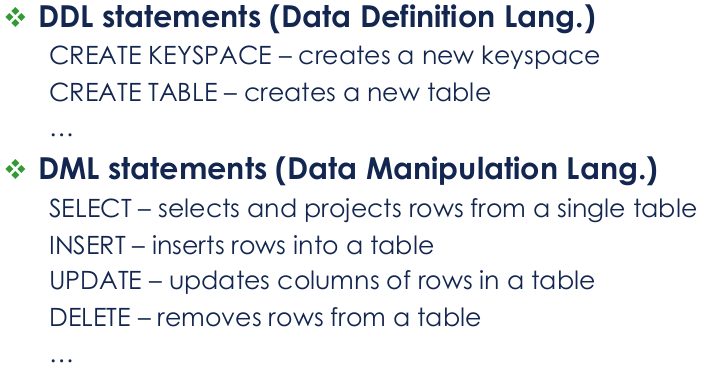
\includegraphics[scale=0.3]{20}
\end{center}

\subsubsection{Keyspace}

\begin{figure}[!h]
  \centering
  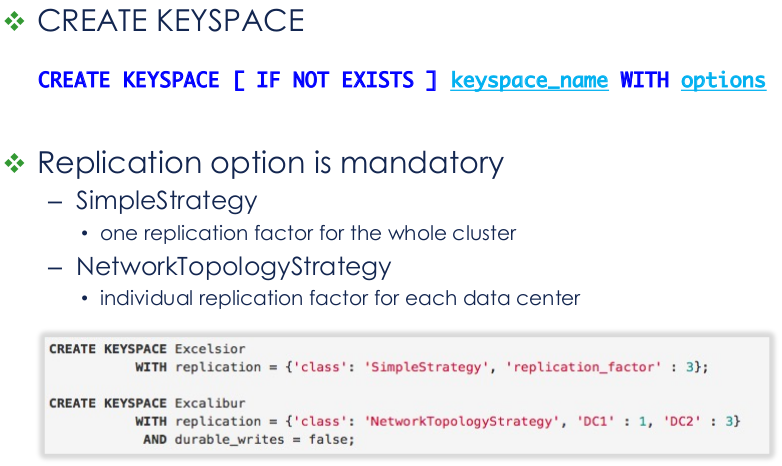
\includegraphics[scale=0.25]{21}
  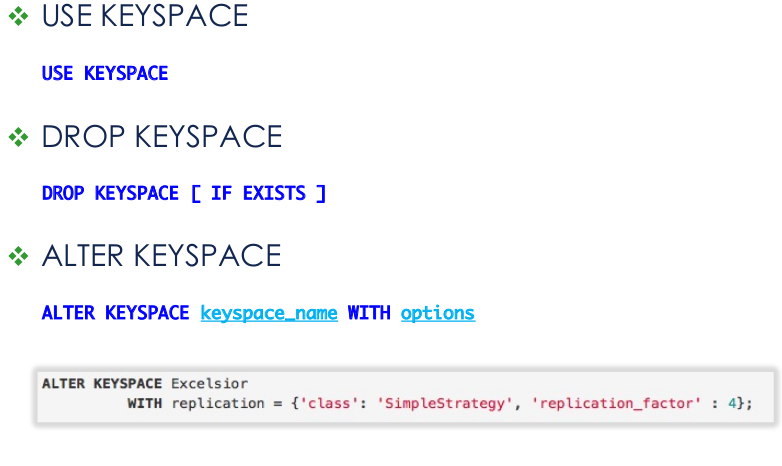
\includegraphics[scale=0.25]{22}
\end{figure}

\pagebreak

\subsubsection{Table - Create Statement}

\begin{center}
  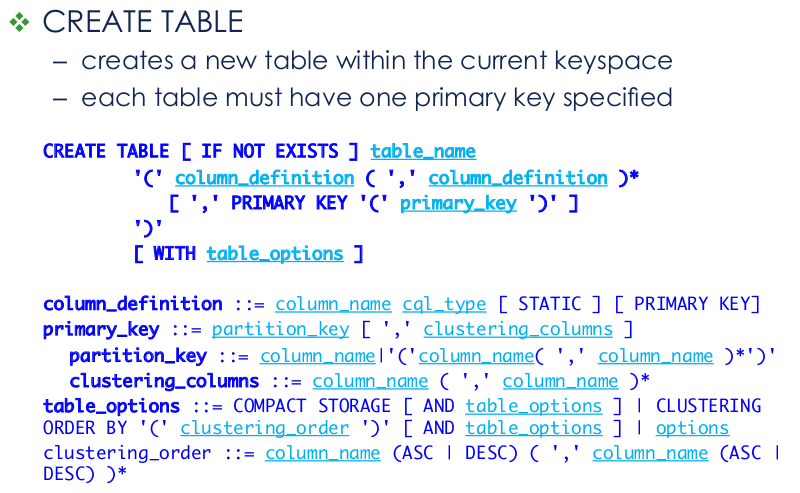
\includegraphics[scale=0.25]{23}
\end{center}

\subsubsection{Table - Primary Key}

\begin{flushleft}
  Primary key has 2 parts:

  \textbf{Compulsory Partition Key:} 
  \begin{itemize}
    \item Uma ou mais colunas;
    \item Descreve como é que as table rows são distribuidas pelas partitions
  \end{itemize}

  \textbf{Optional Clustering Key (ou Columns):}
  \begin{itemize}
    \item Define a Clustering Order, isto é, como é que as tables estão localmente
    guardadas dentro de uma partição;
  \end{itemize}

  \begin{center}
    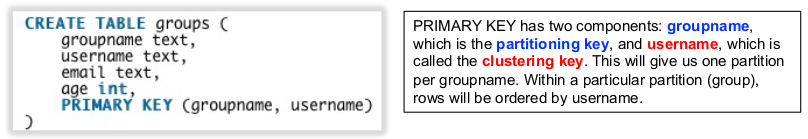
\includegraphics[scale=0.3]{24}
  \end{center}
\end{flushleft}

\subsubsection{Key Roles}

\begin{flushleft}
  \textbf{Partition Key:} Responsável por da Distribution (partitioning)
  pelos nodes da BD. Pode ter multiplas colunas.
  
  \vspace{2mm}

  \textbf{Clustering Key:} Responsável oir Data Sorting dentro de uma partition.
  Pode ter multiplas colunas.

  \vspace{2mm}

  \textbf{Primary Key:} Equivalente a uma Partition Key num Single-Field-Key Table;

  \vspace{2mm}

  \textbf{Composite Key:} Multiple-Column Key

  \begin{figure}[!h]
    \centering
    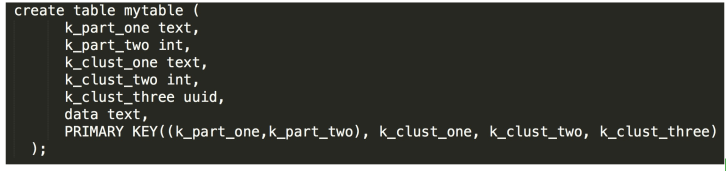
\includegraphics[scale=0.3]{25}
    \caption{Exemplo de uma Composite Key}
  \end{figure}
\end{flushleft}

\pagebreak

\subsubsection{Table - Other Statements}

\begin{center}
  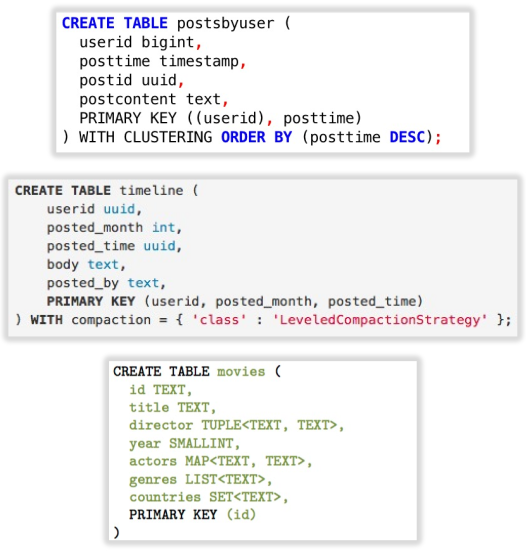
\includegraphics[scale=0.3]{26}
\end{center}

\subsubsection{Select Statement}

\begin{center}
  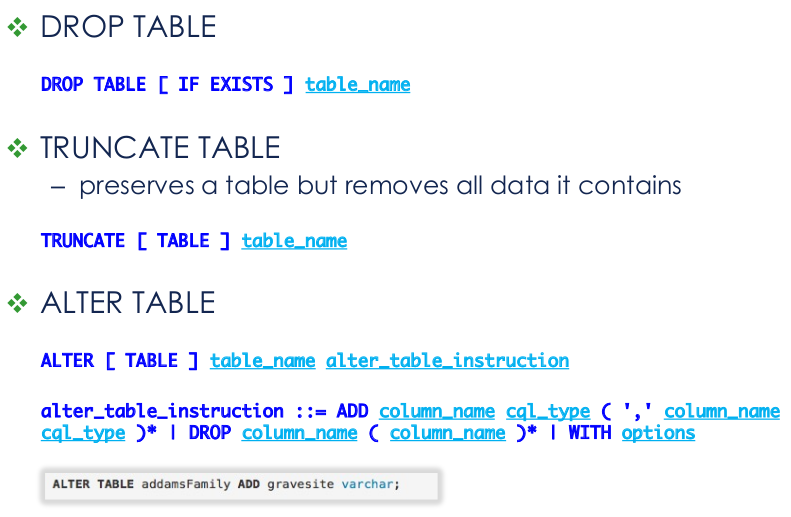
\includegraphics[scale=0.3]{27}
\end{center}

\subsubsection{Select - FROM Clause}

\begin{flushleft}
  Define uma \textbf{única tabela} para a query:
  \begin{itemize}
    \item do keyspace atual/especificado;
    \item \uline{dar join a outras tabelas não é possível};
  \end{itemize}

  \pagebreak

  Suporta:
  \begin{itemize}
    \item \textbf{distinct} para eliminar rows duplicadas;
    \item (user-defined) \textbf{aggregate functions}
    \item \textbf{*} para selecionar todas as colunas;
    \item \textbf{AS} para atribuit um alias a uma coluna;
    \item WRITETIME (timestamp) e TTL (time to live) para selecionar os valores
    de timestamp e ttl de uma coluna (não pode ser usado na clausula WHERE);
  \end{itemize}

  \begin{center}
    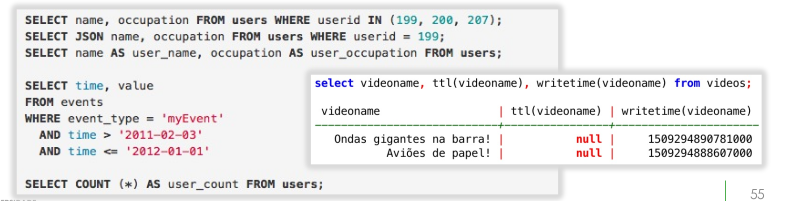
\includegraphics[scale=0.3]{28}
  \end{center}
\end{flushleft}

\subsubsection{Select - WHERE Clause}

\begin{flushleft}
  Sintaxe parecidas entre CQL e SQL.

  As diferenças aparecem devido ao facto da Cassandra estar a lidar com dados
  distribuidos, logo temos de procurar prevenir queries ineficientes
  \begin{itemize}
    \item Rows estão espalhadas pelo cluster baseado na Hash das suas partition keys;
    \item Clustering keys são usadas para fazer cluster dos dados de uma partição
    permitindo um retrieval muito eficiente das rows;
  \end{itemize}

  \vspace{2mm}

  \textbf{Nota:} Partition Key, Clustering e normal columns supostam diferentes
  sets de restrições dentro da clausula WHERE.

  \vspace{2mm}

  \textbf{Partition Key Columns:}
  \begin{itemize}
    \item Suportam \textbf{=} e \textbf{IN};
    \item Todas as primary keys columns tem de ser usadas (restricted),
    a não ser que tenhasmos secondary indexes;
    \item Todas as colunas são precisas para computar a hash que vai permirie localizar
    os nós que contenham os dados partição;
  \end{itemize}

  \vspace{2mm}

  \textbf{Clustering Key:}
  \begin{itemize}
    \item Suportam \textbf{=, $<$, $>$, $<$=, $>$=};
    \item \textbf{IN} retorna verdadeiro se o valor for um dos enumerados;
    \item \textbf{CONTAINS*} e \textbf{CONTAINS KEY}:
    \begin{itemize}
      \item Retornam True se a coleção contiver o dado elemento;
      \item Quando o query estiver a usar um secondary index;
      \item Usado em collections* (lists, sets, maps) / maps**; 
    \end{itemize}
  \end{itemize}
\end{flushleft}

\pagebreak

\subsubsection*{Examples:}

\begin{center}
  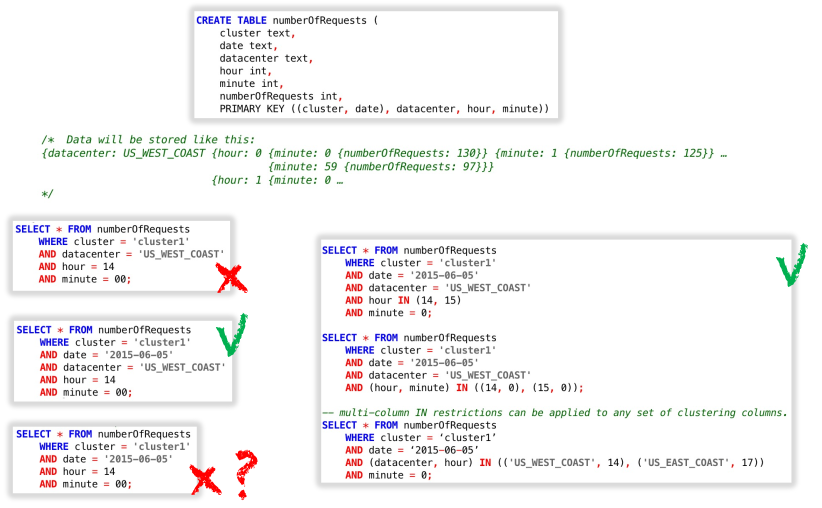
\includegraphics[scale=0.35]{29}
\end{center}

\begin{center}
  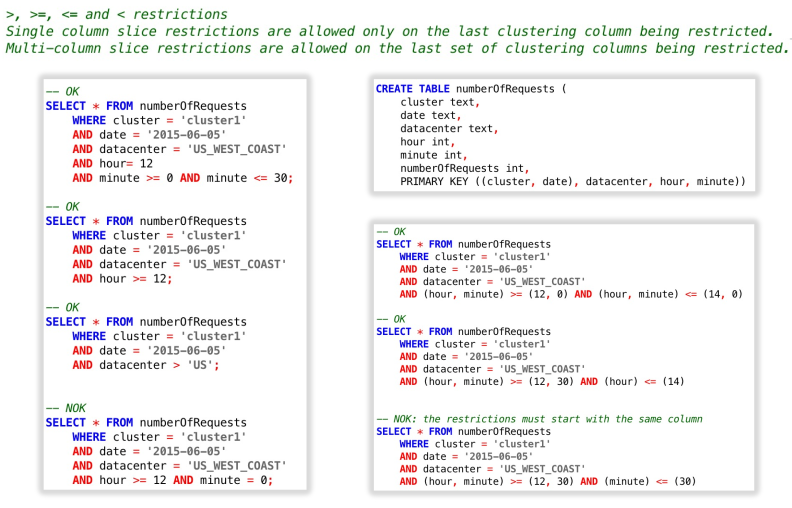
\includegraphics[scale=0.35]{30}
\end{center}

\begin{center}
  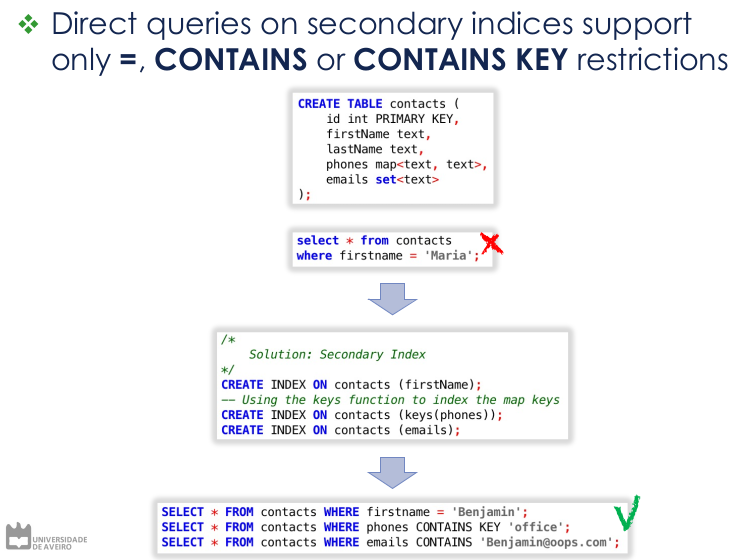
\includegraphics[scale=0.3]{31}
\end{center}

\pagebreak

\subsubsection{Select - GROUP BY, ORDER BY \& LIMIT}

\begin{flushleft}
  \textbf{GROUP BY} clause:
  \begin{itemize}
    \item Agrupar Rows de uma Table de acordo com certas colunas;
    \item \textbf{Apenas grouping induzidos por primary key columns são permitidos};
    \item Quando non-grouping columns são selecionadas sem uma aggregate function,
    o primeiro value encontrado é sempre retornado;
  \end{itemize}

  \vspace{2mm}

  \textbf{ORDER BY} clause:
  \begin{itemize}
    \item Define a ordem (ASC ou DESC) das rows retornadas;
    \item \textbf{Partition Key tem de ser restricted com = ou IN};
    \item \textbf{APENAS} orderings induzidos por \textbf{CLUSTERING COLUMNS} são permitidos;
  \end{itemize}

  \vspace{2mm}

  \textbf{LIMIT} clause:
  \begin{itemize}
    \item Limita o número de rows retornadas numa query result;
  \end{itemize}

  \begin{center}
    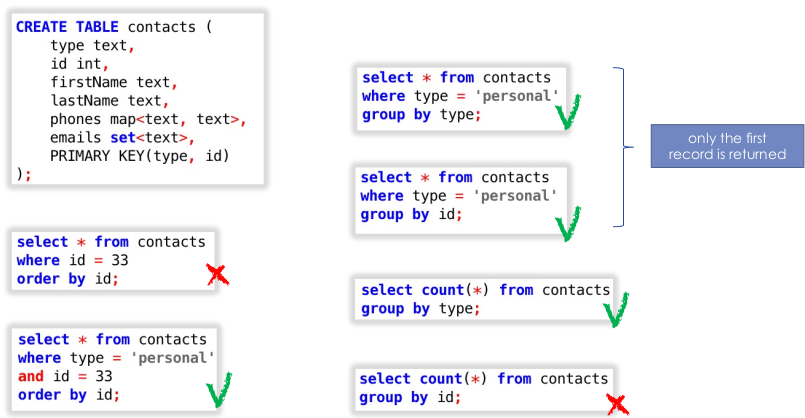
\includegraphics[scale=0.3]{32}
  \end{center}
\end{flushleft}

\subsubsection{Select - User Defined Functions}

\begin{center}
  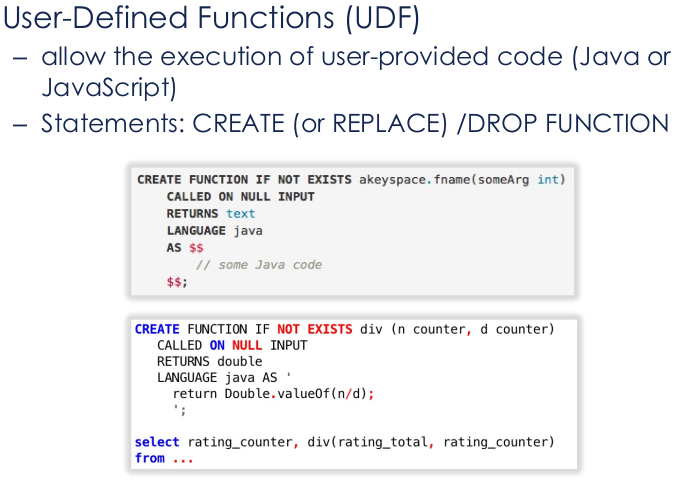
\includegraphics[scale=0.3]{33}
\end{center}

\pagebreak

\subsubsection{Select - Aggregates}

\begin{center}
  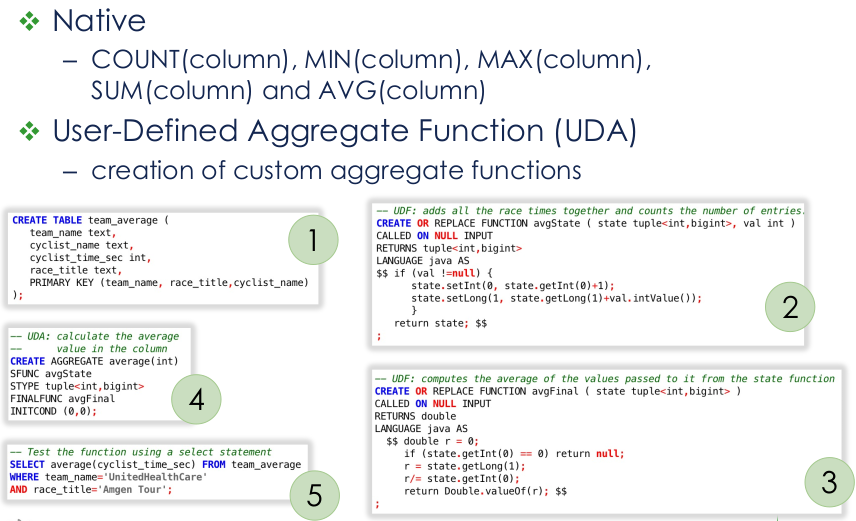
\includegraphics[scale=0.3]{34}
\end{center}

\subsubsection{Select - ALLOW FILTERING}

\begin{center}
  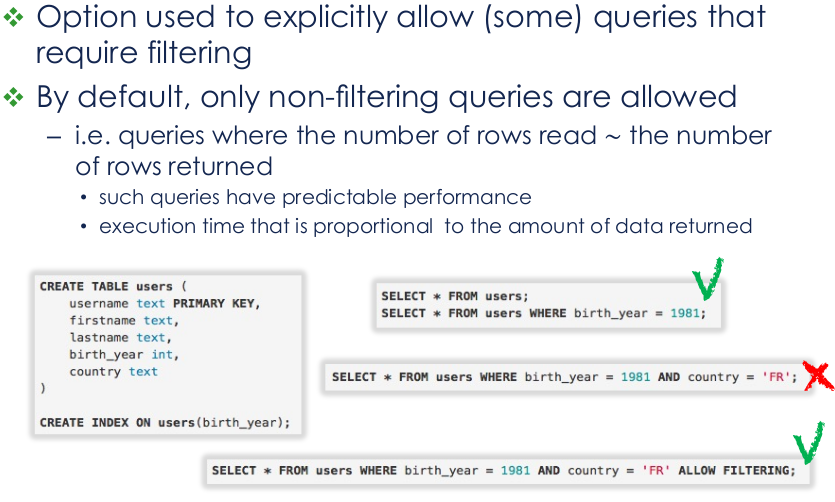
\includegraphics[scale=0.3]{35}
\end{center}

\pagebreak

\subsubsection{Insert Statement}

\begin{flushleft}
  Insere uma nova row numa dada table:
  \begin{itemize}
    \item Se a Primary Key existir, a row é atualizada;
    \item Existe a \textbf{condição IF NOT EXISTS} para apenas inserir caso uma row não exista;
  \end{itemize}

  Escreve uma ou mais colunas para uma dada row.
  Pelo menos as Primeary Key Columns têm de ser especificadas.

  \begin{center}
    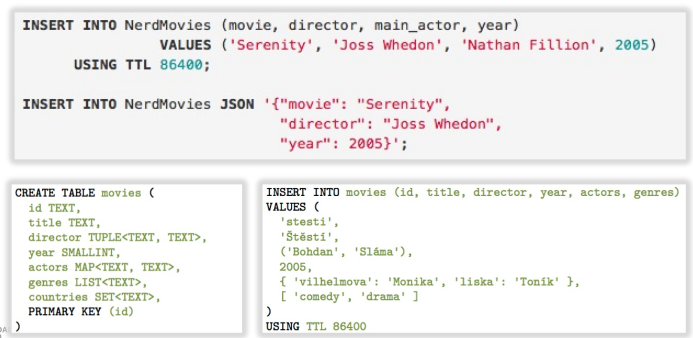
\includegraphics[scale=0.3]{36}
  \end{center}
\end{flushleft}

\subsubsection{Update Statement}

\begin{flushleft}
  Atualiza rows existentes dentro de uma dada table:
  \begin{itemize}
    \item Se a row com a dada primary key não existir, é inserida; 
  \end{itemize}

  Todas as Primary Key Columns têm de ser especificadas na clausula WHERE.

  \begin{figure}[!h]
    \centering
    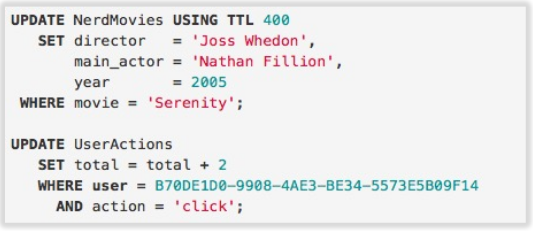
\includegraphics[scale=0.3]{37}
    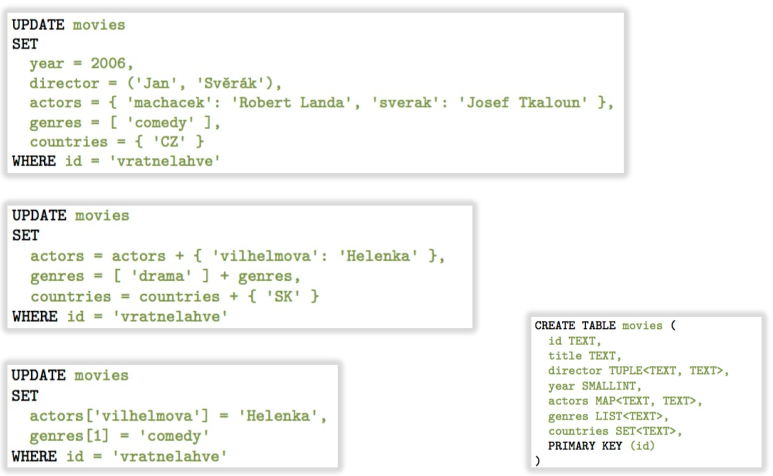
\includegraphics[scale=0.3]{38}
  \end{figure}
\end{flushleft}

\pagebreak

\subsubsection{Parametros Insert \& Update}

\begin{center}
  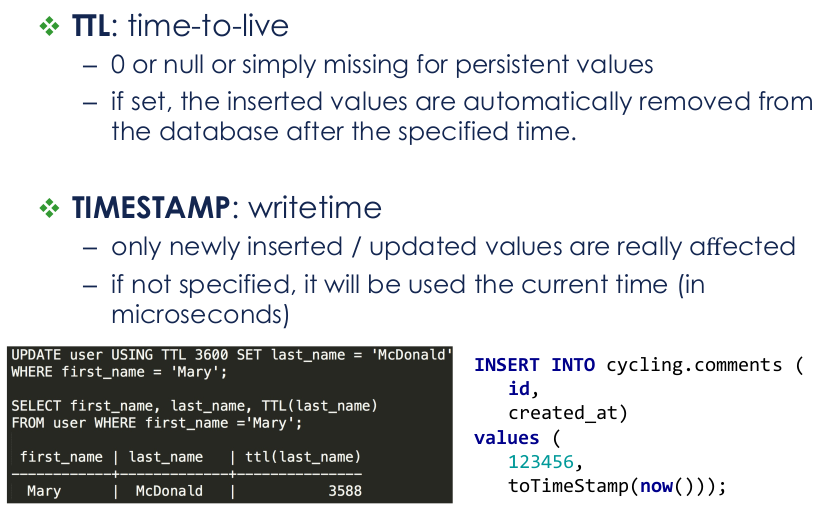
\includegraphics[scale=0.25]{39}
\end{center}

\subsubsection{Delete Statement}

\begin{flushleft}
  Remove existing rows/columns/collection elements de uma dada tabela.

  A clausula \textbf{WHERE} é usada para especificar qual a row que queremos deleted.

  Múltiplas Rows podem ser apagadas com uma única query usando o operador \textbf{IN}.

  Um range de rows pode ser apagado usando um inequality operator ($<$, $>$, $<=$, $>=$).

  \begin{center}
    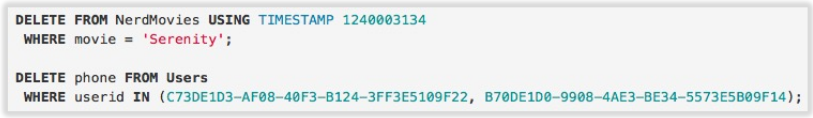
\includegraphics[scale=0.3]{40}
  \end{center}
\end{flushleft}

\end{document}
